\documentclass{article}

\usepackage{amssymb,amsmath,epsfig}
\usepackage{subfigure}
\usepackage{alg}
\usepackage{draftcopy}

\newcommand{\indep}{{\bot\negthickspace\negthickspace\bot}}

\title{MI-toolkit Description}
\author{Karim Filali, Jeff Bilmes\\ \{karim@cs,bilmes@ee\}.washington.edu}

\begin{document}
\maketitle

\begin{abstract}
While many programs are available for calculating information
theoretic quantities, to our knowledge, few are well suited for very
large time series datasets such as speech corpora.  The {\bf Mutual
Information Toolkit} is designed to efficiently calculate such
quantities and be easily parallelizable.

This document describes the MI Toolkit, its purpose,
how it works, and a few of its applications.   
\end{abstract}

\section{Introduction}

%The original purpose of the MI toolkit was to assist in learning
%Graphical Model (GM) structures for automatic speech recognition
%(ASR).  The Hidden Markov Model (HMM) is the simplest and most widely
%used GM in ASR.  In [XX], the HMM is augmented to correct some
%assumptions that it makes but which do not hold in practice.  Finding
%the assumptions that are violated and improving the model is done by
%calculating the {\em mutual information} between different features in
%the speech stream conditioned on given variables.  

%In section XX, we
%detail the structure search approach.

We present this toolkit overview in the context of speech recognition
even though the tools are general enough to be applied to any
time-varying series.

Section~\ref{sec:mi} introduces the background about mutual
information and entropy that is useful for the rest of the discussion.
Section~\ref{sec:toolkit} discusses how the joint probability
distributions are estimated in the toolkit.
%Section~\ref{sec:usage} describes specific options of the toolkit and
%the vector specification syntax.


%The rest of the paper is organized as follows:  In section XX, we describe
%the inputs the toolkit operates on. Section XX provides background on
%the information theoretic quantities we calculate.  Section XX
%describes the internals of the toolkit i.e. the procedures used to
%perform those calculations.   We describe how the toolkit is to be
%used including the command line parameters in section XX.  Finally, we
%talk about some  applications of the tookit in section XX.

\section{Entropy and Mutual Information}
\label{sec:mi}

Mutual information is the amount of information a given random
variable $X$ has about another random variable $Y$
\cite{shannon48,cover91}.  Formally,
\begin{equation}
\label{eq:mi}
I(X;Y)= E_{P_{XY}}[log \frac{p(X,Y)}{p(X)p(Y)}]
\end{equation} 
Mutual information is $0$ when $X$ and $Y$ are independent
(i.e. $p(X,Y)=p(X)p(Y)$) and is maximal when $X$ and $Y$ are
completely dependent i.e. there is a deterministic relationship
between them.  The value of $I(X;Y)$ in that case is $H(X) (=H(Y))$,
where $H(X)$ is the entropy of $X$ and is defined as $H(X) =
E_{P_X}[log(\frac{1}{log(p(X))}]$.  Entropy measures the amount of
uncertainty associated with $X$.

An alternative formulation of MI in terms of entropy is shown in
equation~\ref{eq:entropy}. 

\begin{equation}
\label{eq:entropy}
I(X;Y) = H(X) + H(Y) - H(X,Y);
\end{equation}

where the {\it joint entropy}, $H(X,Y) =
E_{P_{XY}}[log(\frac{1}{log(p(X,Y))}]$.

Neither correlation nor mutual information tell us anything about
causal relationships between variables.  This can be seen, in the case
of MI, from equation~\ref{eq:entropy} where variables $X$ and $Y$ have
symmetric roles.

The definition of the mutual information applies for any random
vectors $X$ and $Y$, but we make the distinction between the {\it
bivariate mutual information}, when $X$ and $Y$ are scalars and {\it
multivariate mutual information}, when $X$ and $Y$ are vectors of
arbitrary dimensions.

Furthermore, we shall refer to quantity $I(X;Y|Z)$ where $Z$ is a
random vector as the {\it conditional mutual information} as opposed
to the { \it unconditional mutual information} $I(X;Y)$.  Similarly to
unconditional MI in equation~\ref{eq:mi}, conditional mutual
information can be written as\footnote{We use capital letters to
denote random variables and lower-case letters to denote specific
values taken by those random variables}

\begin{equation}
\label{eq:cond-mi}
I(X;Y|Z)= \sum_z p(Z=z) E_{P_{XY|z}}[log \frac{p(X,Y|z)}{p(X|z)p(Y|z)}]
\end{equation} 

Conditional mutual information is useful in the context of speech
because it tells us, for example, what the strength of the correlation
between two different features is, given that the features belong to
some class (a vowel, for example).  Another application of conditional
MI is in feature selection, where one might want to select a subset of
a feature vector ${a_1,...,a_{n}}$ and maximize the information that
the subset provides about a given class.  A simple greedy algorithm
adds a feature $a_i$ to the set ${a_{k_1},...,a_{k_m}}$, of previously
chosen features, where $k_i \in {1..n}$ only if
$I(a_j,Q|{a_{k_1},...,a_{k_m}})$, $j \notin {k_1..k_m}$ is highest for
$j=i$.

In the most general case $X$ and $Y$ are continuous variables.
However, because the density estimation methods are different when
either or both of $X$ and $Y$ are continuous, we refer to the case
where both random variables are discrete as {\it discrete MI}.  When
one variable is discrete and the other continuous, we compute the {\it
conditional entropy} $H(X|Q)$ as an intermediate step.  This case is
discussed in section~\ref{sec:toolkit}.

\section{MI Toolkit}
\label{sec:toolkit}

In this section, we describe the type of mutual information quantities
we are interested in computing in the context of discrete time series
in general and speech in particular.  Then we discuss the MI
estimation procedure.

\subsection{Inputs}
\label{sec:inputs}

We can view a finite discrete time series $s(t)$ as a set of
$d$-dimensional vectors or frames indexed by time.  Associated with
each vector, there might also be a ``label,'' a phonetic class label
for example.  We refer to the set of indexed vectors as the {\it
time-series matrix}, an example of which is shown in
figure~\ref{fig:mi-window}.  Each column corresponds to a frame at a
time $t$ and each row corresponds to a feature position.

We assume the input data set is divided into {\em sentences}, each of
which is a sequence of {\em frames}.  At any given time, a single
sentence is loaded into memory.  The maximum amount of memory required
can therefore be controlled by restricting the length of sentences.

Besides the data, an input to the MI tools are the specifications of
the relative positions of the features in the speech frames, between
which we want to compute the MI.  At any given time/frame, such a
specification defines two vectors $X$ and $Y$.  By going over the
data, we collect instances of vectors $X$ and $Y$.

For example, as depicted in figure~\ref{fig:mi-window}, one might want
to know the strength of the dependency between a feature position in
two consecutive frames, on one part, and its left and right contexts
on the other.  The syntax used to write the specification above is
\begin{verbatim} [3@0;3@-1] [3@-2;3@1] \end{verbatim}

\begin{figure}
\center
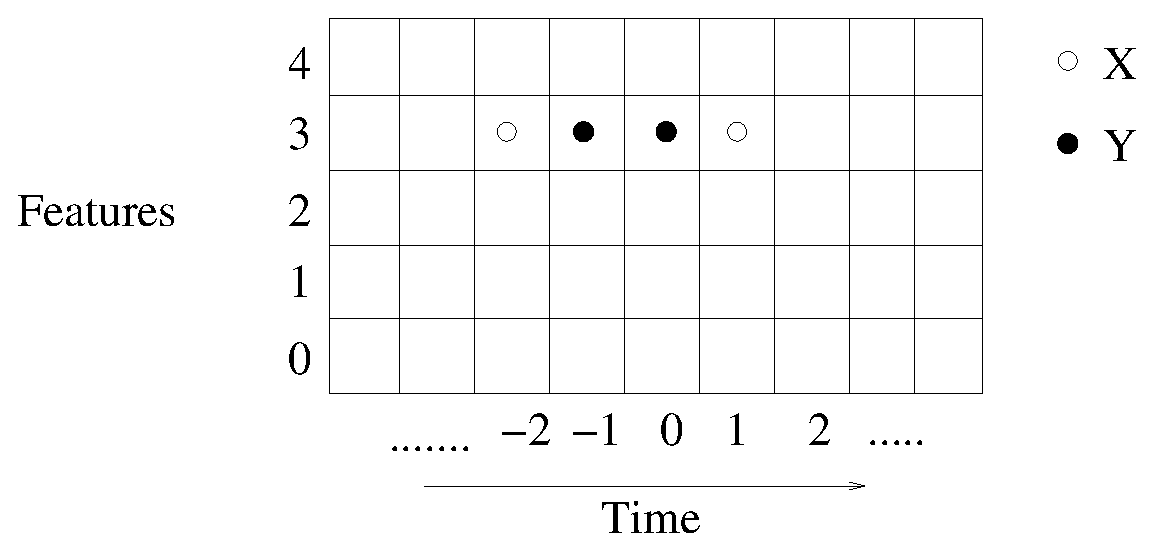
\psfig{file=mi-window.eps,width=6.0cm}
\caption{\label{fig:mi-window} A time series matrix.  Shown are two
sets $X$ and $Y$ of feature-lag coordinates.  $I(X;Y)$ here would tell
us how much information there is between two consecutive features at
position 3 and their left and right contexts.  Where the time origin
is set does not matter in the unconditional case.  It does matter when
calculating $I(X;Y|Q)$ as the $X$ and $Y$ samples are collected such
that the class of the zero-lag feature is $Q$.}
\end{figure}


%% While the mutual information value for a given pair of random vectors
%% can be useful in itself to assess whether there is any correlation, it
%% is often more useful to compare it across all possible all features
%% and time lags.  In the example of figure~\ref{fig:mi-window}, we might
%% want to compute the MI using the same time-lag configuration but for
%% all feature positions.  Or, vary the lag of the left and right
%% contexts.  A particular useful visualization of bivariate MI between
%% feature pairs is depicted in figure~\ref{fig:mi-window2}: a
%% feature-lag window is chosen and MI is computed for all child-parent
%% feature combinations, where ``child'' refers to a feature at lag 0 only,
%% and ``parent'' any feature within that window, including at lag 0.
%% Section~\ref{sec:exps} discusses how we can use projections to
%% visualize the resulting four-dimensional graph of MI versus child and
%% parent features and time lag.

%% \begin{figure}
%% \psfig{file=mi-window2.eps,width=6.0cm}
%% \caption{\label{fig:mi-window2} Time series matrix with a feature-lag
%%   window of size 5x2.  Arrows point from all possible parent features
%%   to all children.  For clarity not all arrows are shown.}
%% \end{figure}


\subsection{Density Estimation}

There are two main steps to calculate mutual information.  First, the
joint probability distribution $P_{XY}$ for $X$ and $Y$ is estimated.
When all the random variables are discrete, this estimation is straight
forward and involves finding the frequency of each discrete value of
$X$ and $Y$.  In the continuous case, histogram-based methods reduce
the problem to the discrete case by partitioning the continuous ranges of
$X$ and $Y$ into bins.  Parametric methods assume some distribution
type for $P_{XY}$ and try to learn its parameters.  A popular
distribution is a mixture of Gaussians because it yields closed-form
formulae for the Expectation Maximization estimation of the parameters
and makes the marginalization operations (obtaining $P_X$ and $P_Y$
from $P_{XY}$) straight-forward.

A disadvantage of the parametric method is the Gaussian assumption
that it makes; a different type of distribution---heavy-tailed for
example---might be more appropriate especially in light of the results
showing the strong non-Gaussian character of speech data. An
advantage, however, of the approach is that it requires less data
(\cite{morris92}) and is not susceptible to the same bias problem
non-parametric methods suffer from.  The MI toolkit uses a parametric
estimation method.

The second step is the computation of the mutual information value
from $P_{XY}$ and the marginals $P_X$ and $P_Y$.  We can use
equation~\ref{eq:mi} or the alternative form in equation~\ref{eq:entropy}.

We use three different ways to estimate the entropy quantities in
equation~\ref{eq:entropy}:  
\begin{enumerate}\addtolength{\itemsep}{-0.6\baselineskip}
\item Sampling from the learned distribution 
\item Sampling using the data
\item Grid method (only used in the bivariate MI program)
\end{enumerate} 

The first method relies on the law of large numbers:
\begin{eqnarray*}
\lim \frac{1}{N}\sum_{i=1}^N p(x_i) log(p(x_i)) &=& E_{P_X}[log(p(x)] \\
						&=& -H(X)
\end{eqnarray*}

As the number of samples $N$ increases, $\frac{1}{N}\sum_{i=1}^N
p(x_i) log(p(x_i)) $ tends to the true expectation $E_{P_X}[log(p(x)]$.

Sampling using the data means that the same data that was used to
learn the distribution are used to generate the samples to estimate
entropies.  This method is used only for computational reasons.  If
not enough data is used, the MI values might not be accurate (they can
turn out negative for example).

The grid method subdivides the probability space into histogram bins,
calculates the probability associated with each bin (usually the
probability of the center) and multiplies by the bin size summing over
all bins.  This is very similar to numerical integration of a
two-variable function.  There is a trade-off between a small size of the
size of the bins--and thus more bins--which a more accurate density
estimate and the fewer bins which speeds up computation.

\subsection{MI Calculation}

This section describes the full procedure (algorithm~\ref{alg}) to
compute mutual information values from data over a given feature-lag
window.

The main element of the estimation algorithm is the Expectation
Maximization procedure, which starts by hypothesizing the parameters
of the distribution and after each iteration learns new parameters by
maximizing the likelihood of the data given the previous parameters.
Since we are using mixtures of Gaussians, there are three parameters
to learn: means, covariance matrices and weights of Gaussian
components.

\begin{algorithm}[ht]
\label{alg}
\caption{Compute MI(S, T)}
\alginout{$S$ is the set of $n$ sentences ${S^{(1)}...S^{(n)}}$.\\
$T$ is a set of $m$ pairs $(X^{(i)},Y^{(i)})$, $i=1..m$ for which we want to compute MI, where
$X$ and $Y$ are vectors of feature-lag coordinates.  $T^{(i)}$ refers to
the $i$th pair and is said to be active if its difference in
likelihood from the previous iteration is greater than some threshold.
}{Outputs the MI for each
$(X,Y)$ pair.\\}
\begin{algtab}
\algwhile{Some pair is active}
%$i \leftarrow 1$\\
%\algwhile{$i < n$}	
\algforto{$i=1$}{$n$}
   Read $S_i$\\
   \algforto{$j=1$}{$m$}
       \algif{$T^{(j)}$ is active}
	   Form a vector $V$ of the entries with coords
$(X^{(j)},Y^{(j)})$\\  
	   Accumulate sufficient statistics\\
       \algend	
    \algend
\algend
Update means, covariance matrices and weights of all active mixtures.\\
\algend
\algforto{$j=1$}{$m$}
   Obtain $p_X^{(j)}$ and $p_Y^{(j)}$ by marginalizing the joint distribution $P_{XY}^{(j)}$\\
   Sample from the joint and the marginal distributions to calculate the entropy values $H(X)$, $H(Y)$ and  $H(X,Y)$\\
\algend
\end{algtab}
\end{algorithm}

The marginalization step consists of partitioning the mean vectors and
covariance matrices according to the partition of the vector $V$.
Sampling in the last step of the algorithm can be replaced by the grid
method described above.  We only use the grid method in the bivariate
case because as the dimensionality of $V$ increases the ``grid'' size
increases as well and its computational advantage over the sampling
method disappears. 

\subsection{Mixed Continuous-discrete Variables}
\label{subsec:mixed}

Often we are interested in the mutual information between a continuous
and a discrete variable i.e. we want to calculate $I(X,Q)$ where $X$
is continuous and $Q$ discrete.  Such a calculation is needed, for
example to compute the amount of MI between a set of features and
phonetic indices or to augment the feature set in a graphical model
with a second set of features independent of the phone but dependent on
the first feature set \cite{zweig2002}.

We can write the mutual information as a function of entropy and we get

\begin{eqnarray}
\label{eqnarray:mixed}
I(X,Q) 	&=& H(X) - H(X|Q) \\
	&=& E_p[\frac{1}{\log(p(X))}] - E_{p(x,q)}[\frac{1}{\log p(X|Q)}]
\end{eqnarray}

The term $H(X|Q)$ can be further expanded:

\begin{equation}
\label{eq:mixed}
H(X|Q)=-\sum_{q_i} p(q_i) E_{p(x|q)}[\log p(X|Q=q_i)]
\end{equation}

From equation~\ref{eq:mixed}, there are two probability distributions
that we need to estimate:  $p_Q$ and $p_{X|Q}$.  The density
$p_{X|Q}$ is estimated the same as $p_X$ except the data points $X$
are drawn from frames of class $Q$.  $p_Q$ is just the (discrete)
class distribution. 

Note that in equation~\ref{eqnarray:mixed} we could have conditioned the
entropy on the continuous variable instead of the discrete one.  However,
a restriction of the MI toolkit is that conditioning on a continuous
variable is not yet supported.  Doing so would require either
to discretize the conditioned-upon continuous variable or to learn the
conditional entropy quantity using a neural network for example.

\subsection{Vanishing Gaussian Components}

A mixture of weighted Gaussians components can approximate any
distribution arbitrarily well for a large enough number of Gaussians.
It is, however, not computationally practical to use a large number of
components; moreover, it is often the case that a only few Gaussians
will account for most of the probability mass of the distribution.
One way to speed computation without affecting the accuracy of the
density estimation is to vanish those components which weights
relative to uniform weights fall below some threshold.

\subsection{Implementation Example}

Below we describe an example of how to compute a mutual information
quantity, which broken down into its component parts, can be computed
using the MI toolkit.

Suppose we are interested in computing the quantity
$I({C_1,C_2,D_1,D_2};{C_3,C_4,D_3} )$.  By successive use of the
formula (where the roles of $X$ and $Y$ can be reversed)
\begin{equation}
I(X;Y_1,Y_2)= I(X;Y_1) +I(X;Y_2|Y_1)
\end{equation}

we get
\begin{eqnarray*}
\lefteqn{I(\{C_1,C_2,D_1,D_2\};\{C_3,C_4,D_3\} )} \\ 
&=& I(\{D_1,D_2\};\{C_3,C_4,D_3\}) \\
& & \mbox{} + I(\{C_1,C_2\};\{C_3,C_4,D_3\}|\{D_1,D_2\}) \\
&=& I(\{D_1,D_2\};D_3) \\
& & \mbox{} + I(\{D_1,D_2\};\{C_3,C_4\}|D_3) \\
& & \mbox{} + I(\{C_1,C_2\};D_3|\{D_1,D_2\}) \\
& & \mbox{} + I(\{C_1,C_2\};\{C_3,C_4\}|\{D_1,D_2,D_3\})
\end{eqnarray*}

In all four terms in the last equation only discrete variables are
present on the right of the conditioning bar.  All four terms can
be computed using the toolkit.


%% \subsection{Parallelism}

%% One of the main difficulties of computing mutual information
%% systematically over a feature-lag window (cf. \ref{fig:mi-window2}) is
%% the exponential increase in the number of parent(s)-child tuples as
%% the number of parents per child (and thus the dimensionality of the
%% random vector $X$, assuming $X$ is the parent feature vector and $Y$
%% the child variable) increases.  In the bivariate case---the simplest
%% case---the number of tuples is $D*L$ where $D$ is the dimension of the
%% observation vector and $L$ the maximum lag i.e. the feature-lag window
%% has dimensions $D*L$.  In the trivariate case, there are $D* {D \times
%% L} \choose 2$ tuples and in general the number of tuples is in the
%% order $\O(L^n \times D^{n+1})$ where $n$ is the dimension of $X$ (the
%% parent vector) and, without lack of generality, is assumed less than
%% $DL/2$.  A concrete example of the large number of tuples in the
%% trivariate case using typical values we use for our bivariate
%% experiments is $D=26, L=15, n=2$, which yields
%% approximately~\footnote{At lag 0, some tuples are not possible because
%% no repetition is allowed within a tuple.} $2000000$ possible tuples
%% (compared to $10816$ for $n=1$).

%% Because of the high computational cost, a primary design goal of the
%% MI toolkit is easy parallelization, which is achieved by splitting the
%% set of all possible tuples and running separate instances of the MI
%% program on a different subset of tuples.  The finest degree of
%% parallelism is achieved when the size of the subsets is one.  This
%% parallelism does not require any communication between different
%% instances of the program---as would be the case if parallelism were
%% achieved via splitting the data.  


% section{Applications}

% subsection{Learning Buried Markov Models}

% subsection{Analyzing Data Dependencies in Different Accoustic Features}

% subsection{Learning Optimal Subvector Partioning for VQ}

\bibliographystyle{plain} { \scriptsize
\bibliography{/homes/karim/bib/bib} }

\end{document}
